\section{Theoretischer Hintergrund}
\label{sec:Theorie}
\subsection{Grundlegende Beschreibung von Kristallstrukturen}
Kristalle sind räumlich periodische Gitter, die durch die Verbindung der zugrunde liegenden Materialien besteht. 
Die kleinste Einheit dieses Gitters wird Basis genannt, welche durch drei Gittervektoren $\vec{a}$, $\vec{b}$ und $\vec{c}$ aufgespannt wird.
Die Struktur des Gitters ist durch die Basis dann eindeutig festgelegt und heißt Elementarzelle.
Ohne weitere Eigenschaften festzulegen gibt es unendlich viele Punktgitter.
Zwei 2D-Gitter sind in Abbiildung \ref{fig:2dgitter} dargestellt.
\begin{figure}
	\centering
	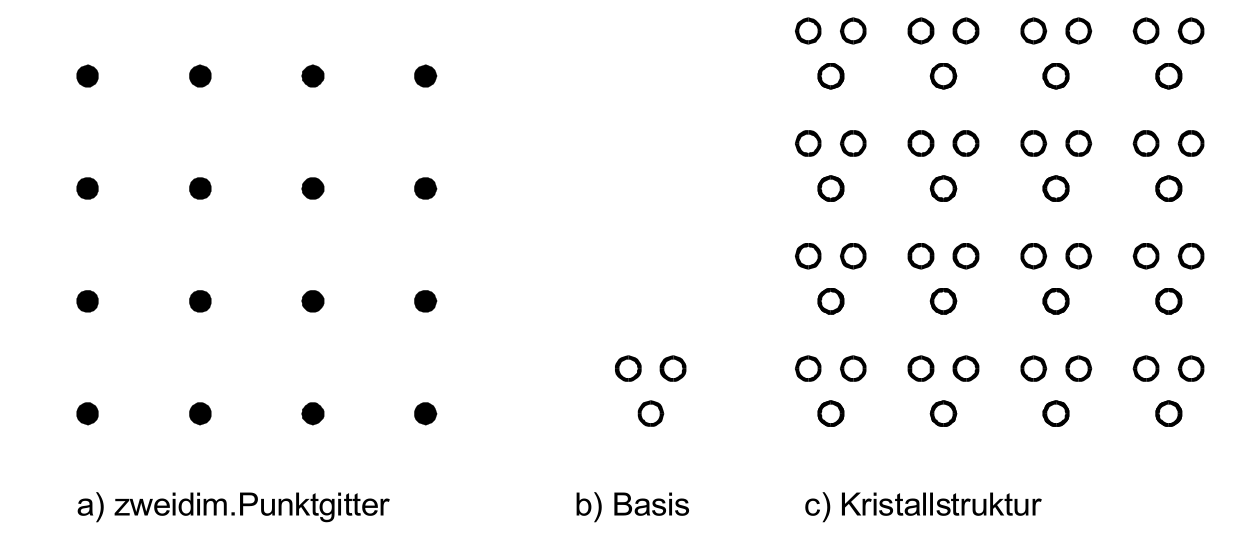
\includegraphics[width = \textwidth]{Abbildungen/2dgitter.png}
	\caption{Zeigt die Unterschiede zwischen Gitter, Basis und Kristallstruktur \cite{Anleitung}.}
	\label{fig:2dgitter}
\end{figure} 
Damit die Gitter klassifiziet werden können, wird die Invarianz unter Symmetrieeigenschaften getestet. \\
Die einfachste erhaltene Symmetrie, die einen Kristall auszeichnet ist die fundamentale Translation. Das bedeuetet, dass ein Vektor $\vec{t}$ durch die folgende Bedingung in Gleichung \ref{eq:fundamentale trans} aus den Basisvektoren darstellbar ist.
\begin{equation}
\vec{\text{t}} = n_1 \vec{\text{a}}+n_2 \vec{\text{b}}+n_3 \vec{\text{c}}
\label{eq:fundamentale trans}
\end{equation}
Die Vorfaktoren der Basisvektoren sind Elemente der natürlichen Zahlen $\mathbb{N}$.
Beistzt das Parallelepiped, welches durch die drei Basisvektoerne aufgespannt wird, nur in jeder Ecke ein Atom, so wird diese Zelle primitiv gennant.
Da nur der Anteil des Atoms, der innerhlab des Epipeds liegt, zählt, besteht die primitive EInheistzelle aus einem Atom.
Das ist die simpelste Form einer Zelle. 
Die weiteren Punktgitter, die durch die Symmetrieoperationen der Inversion, Spiegelung und Rotation klassifiziert werden, teilen sich in 14 Gittertypen auf. 
Diese heißen Bravais-Gitter und können in sieben Kristallsysteme, wie in Abbildung \ref{fig:System} unterteilt werden.
\begin{figure}
	\centering
	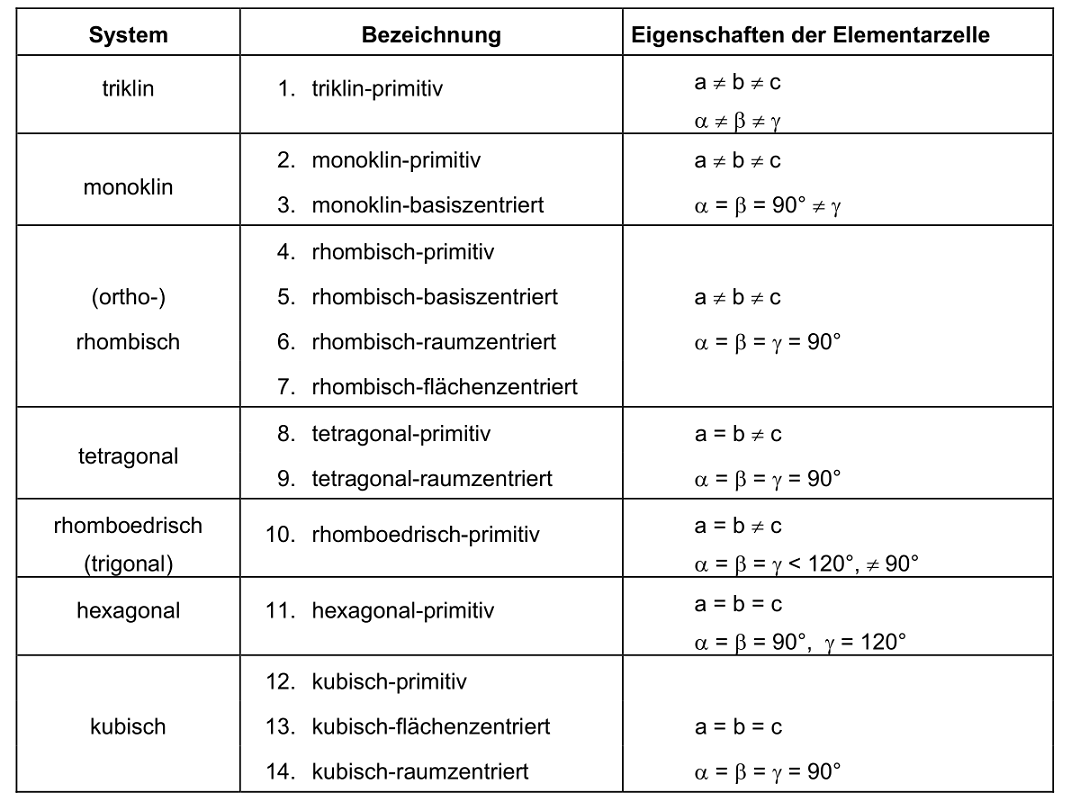
\includegraphics[width = \textwidth]{Abbildungen/System.png}
	\caption{Die Bravais-Gitter aufgeteilt in ihre Kristallsysteme mit den dazugehörigen Eigenschaften \cite{Anleitung}}
	\label{fig:System}
\end{figure} 
\subsection{Das kubische Kristallsystem}
Für die in diesem Versuch untersuchten Materialien ist insbesondere die kubische Gitterstruktur relvant, da Metalle und Salze vorzugsweise kubisch aufgebaut sind.
Das kubische System ist in drei Klassen eingeteilt.\\
Die simpelste Struktur weist das kubisch primitive Gitter auf, welches aus einem Atom besteht und die primitive Einheitszelle in Würfelform beschreibt.
Aus zwei Atomen pro Einheitszelle besteht das kubisch raumzentrierte Gitter, welches als Grundmodell die primitive Einheitszelle besitzt und zusätzlich in der Mitte des Würfels noch ein weiteres Atom besitzt.
Doppelt so viele Atome wie die das kubisch-raumzentrierte Gitter besitzt das kubisch-flächenzentrierte Gitter.
Hier liegt bei dem einfach kubische Gitter auf jeder Würfelfläche noch ein weiteres Atom.
Beispiele für die zuletzt genannten Gittertypen sind in Abbildung \ref{fig:gittertypen} gegeben.

\begin{figure}[h]
	\begin{minipage}[t]{0.45\textwidth}
		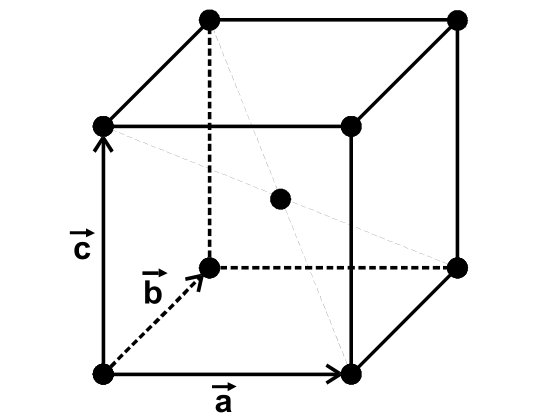
\includegraphics[width=\textwidth]{Abbildungen/raumzentriert}
		\subcaption{Das kubisch-raumzentrierte Gitter hat 2 Atome an den Orten (0,0,0) und $\left(\frac{1}{2}, \frac{1}{2}, \frac{1}{2} \right)$ und 8 nächste Nachbarn im Abstand von $\frac{1}{2}\sqrt{3}$a.}
	\end{minipage}
	\begin{minipage}[t]{0.45\textwidth}
		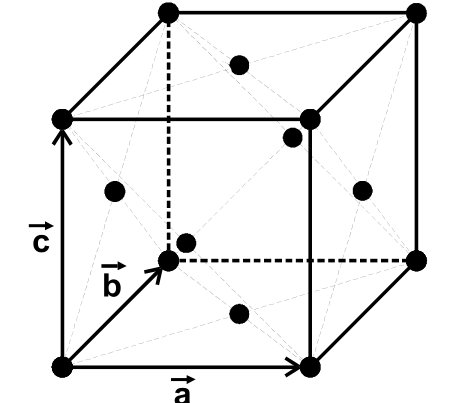
\includegraphics[width=\textwidth]{Abbildungen/flaechenzentriert}
		\subcaption{Das kubisch-flächenzentrierte Gitter hat 4 Atome an den Orten (0,0,0), $\left(\frac{1}{2}, \frac{1}{2}, 0 \right)$, $\left(\frac{1}{2}, 0, \frac{1}{2} \right)$, $\left(0, \frac{1}{2}, \frac{1}{2} \right)$  und besitzt 12 nächste Nachbarn im Abstand von $\frac{1}{2}\sqrt{2}$a.   }
\end{minipage}
\caption{Die Elementaren kubischen Gittertypen bei denen gilt $|a|=|b|= |c|$. \cite{Anleitung}}
\label{fig:gittertypen}
\end{figure}

In der Natur kristallieren Metalle und Salze nicht in einer so simplen kubischen Struktur. 
Die häufigste Struktur ist die Diamantstruktur. 
Sie besteht aus  zwei kubisch-flächenzentrierten Gittern die um ein viertel der Raumdiagonalen zueinander vorschoben sind. 
Es folgt, dass die Diamantstruktur acht Atome an den Orten
\begin{equation}
(0,0,0), \left(\frac{1}{2}, \frac{1}{2}, 0 \right), \left(\frac{1}{2}, 0, \frac{1}{2} \right), \left(0, \frac{1}{2}, \frac{1}{2} \right), \left(\frac{1}{4}, \frac{1}{4}, \frac{1}{4} \right), \left(\frac{3}{4}, \frac{3}{4}, \frac{1}{4} \right), \left(\frac{3}{4}, \frac{1}{4}, \frac{3}{4} \right),  \left(\frac{1}{4}, \frac{3}{4}, \frac{3}{4} \right)
\end{equation}
in der Einheitszelle aufweist.
Die vier nächsten Nachbarn jedes Atoms liegen auf einer Tetraeder Struktur um das Atom herum.
Dies entspricht der sp$^3$-Hybridiesierung des Kohlenstoffs und ist auch in Silizium und Germanium zu finden.\\
Die Diamantstruktur unterscheidet sich von der Zinkblende nur dadurch, dass die Zinkblende aus zwei unterschiedlichen Atomen besteht, die getrennt auf die jeweiligen fcc-Strukturen verteilt sind.\\
Salze kristallieren dahhingegen vielfältiger.
Es werden drei Arten vorgestellt.\\
Die erste ist die Steinsalz-Struktur. 
Sie ist wie die Diamantstruktur, wobei die fcc-Gitter diesmal um eine halbe Raumdiagonale gegneinander verschoben sind\\
Im Gegensatz dazu besteht die Casiumchlorid-Struktur aus zwei primitiven Gittern, die um eine halbe Raumdiagonale gegeneinander verschoben sind. 
Es entspricht der bcc-Struktur, wobei das Atom in der Mitte des Würfels nun ungleich dem am Rand ist.\\
Zuletzt wird noch die Fluorit-Struktur beschrieben.
Sie besteht aus drei fcc-Gittern, die jeweils um eine viertel Raumdiagonal gegeneinander verschoben sind. 
Das heißt, dass die Einheitszelle 12 Atome besitzt.\\\\
Die am dichtesten gepackte Kugelpackung, bei der gerade noch so Platz für alle Atome ist, ist in hexagonalen Gittern zu finden. 
Grundlage der hexagonalen Struktur, wie in Abbildung \ref{fig:hexagonal} zu sehen ist bilden die Raute mit $120\circ$  Winkeln.
\begin{figure}[h]
	\centering
	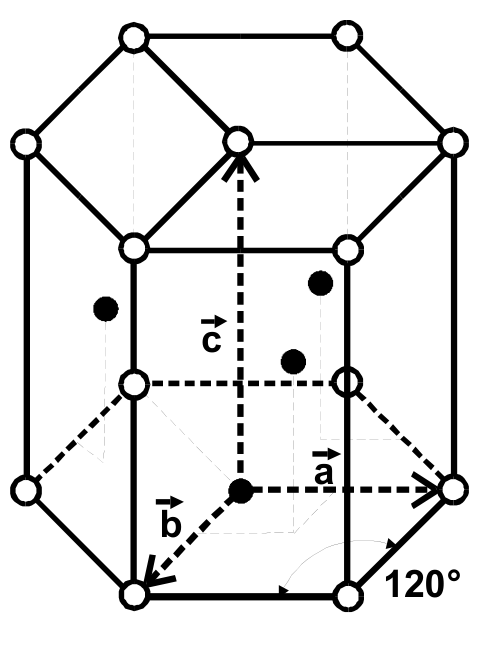
\includegraphics[width = 0.3\textwidth]{Abbildungen/hexagonal.png}
	\caption{Hexagonale Einheitszelle mit den Basisvektoren \cite{Anleitung}. }
	\label{fig:hexagonal}
\end{figure} 
Charakteristisch für die dichteste Kugelpackung ist das Achsenverhätnis von c/a = $\sqrt{\frac{8}{3}}$ wobei der Betrag der Basisvektoren $\vec{a}$ und $\vec{b}$ gleich sind.

\subsection{Millersche Indizes und Netzebenenabstand}
Wenn in einer Ebene die Schwerpunkte von Atomen eines Gitters liegen, so ist diese Ebene eine Netzebene.
Die millerschen Indizes werden durch die Netzebenen aufgestellt. 
Sie sind durch die Form (hkl) charakterisiert, wobei jede Zahl der Reziprokwert der Zahl ist, bei der die Netzebene eine der Achsen schneidet. 
Dies wird in Abbildung \ref{fig:miller} durch die beispielhafte Netzeben deutlich.

\begin{figure}[h]
	\begin{minipage}[t]{0.45\textwidth}
		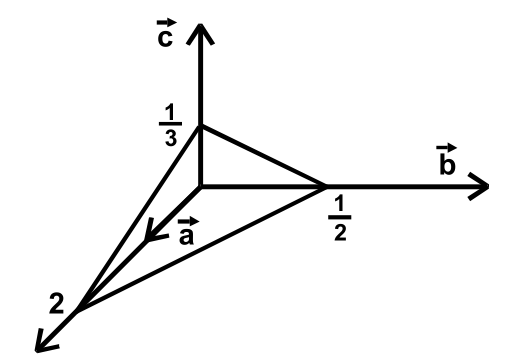
\includegraphics[width=\textwidth]{Abbildungen/miller}
		\subcaption{Netzebene mit den Millerindizes (146)}
	\end{minipage}
	\begin{minipage}[t]{0.45\textwidth}
		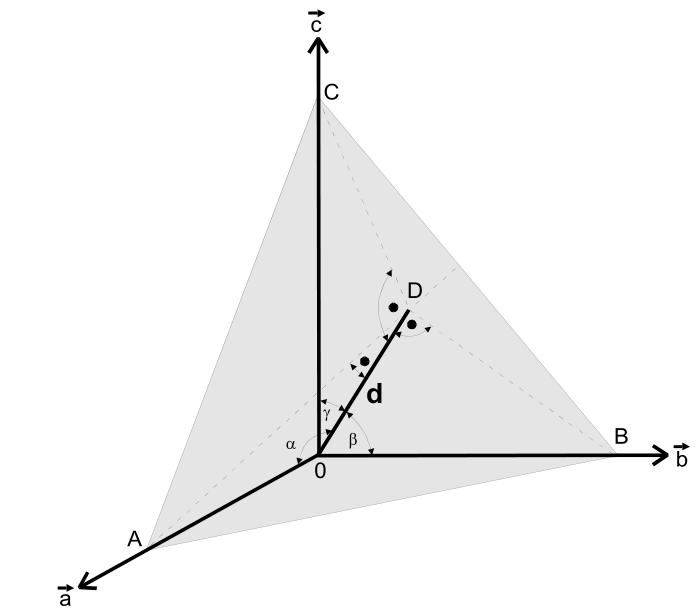
\includegraphics[width=\textwidth]{Abbildungen/netzebene}
		\subcaption{Schematische Darstellung des Netzebenenabstands d einer belibig gewählten Netzebene}
	\end{minipage}
	\caption{Beispielhafte Netzebenen zur Bestimmung der Millerindizes und des Netzebenenabstandes \cite{Anleitung}. }
	\label{fig:miller}
\end{figure}

Tritt der Fall auf, dass eine Netzeben im euklidischen Raum nur eine Achse schneidet, und die anderen beiden nicht, also der Wert $\infty$ ist, so ist der reziproke Wert 0. 
Beispiel für diesen Fall sind die Würfeloberflächen eines kubischen Gitters. 
Die obere Seite hat die Millerindizes (001).\\\\
Der Abstand einer Ebene zum Ursprung des Koordinatensystems wird durch den Netzebenenabstand d angegeben.
Der Netzebenanbstand ist der Betrag des Vektors $\vec{d}$, der stets senkrecht auf der Ebene steht und den Null-Punkt des Koordinatensystems mit dem der Ebene verbindet, wie in Abbildung \ref{fig:miller} gezeigt.
Alle höheren Netzebenen, die parallel zur ersten sind, haben genau den Abstand d voneinander.
Der Netzebenenabstand berechent sich wie folgt.
Die Dreiecke ODA, ODB, ODC in \ref{fig:miller} stehen senkrecht zueinander. Daraus folgt, dass
\begin{equation}
\cos{\alpha} = \frac{\text{d}\text{h}}{\text{a}}, \cos{\beta} = \frac{\text{d}\text{k}}{\text{b}}, \cos{\gamma} = \frac{\text{d}\text{l}}{\text{c}}
\label{eq:Abstand1}
\end{equation}
 und es gilt zusätzlich
\begin{equation}
\cos{\alpha}^2+\cos{\beta}^2+\cos{\gamma}^2 = 1
\label{eq:Abstand2}
\end{equation}
Werden nun die Gleichungen \ref{eq:Abstand1} und \ref{eq:Abstand2} ineinander eingesetzt, so ergibt sich für den Netzebenenabstand Gleichung \ref{eq:Abstand3}
\begin{equation}
\text{d} = \frac{1}{\sqrt{\frac{\text{h}}{\text{a}}^2+\frac{\text{k}}{\text{b}}^2+\frac{\text{l}}{\text{c}}^2}}
\label{eq:Abstand3}
\end{equation}
Ist das System kubisch, so gilt a = b = c und Gleichung (\ref{eq:Abstand4}).
\begin{equation}
\text{d} = \frac{\text{a}}{\sqrt{\text{h}^2+\text{k}^2+\text{l}^2}}
\label{eq:Abstand4}
\end{equation}

\subsection{Röntegnbeugung an Kristallen}
Röntgenstrahlen sind hochenergetische elektromagnetische Wellen, deren Wellenlänge im Bereich Angström liegt. 
Beim Eintritt in einen Kristall treten sie mit den Atomen in Wechselwirkung und werden im klassischen Sinne gestreut.
Die geladenen Teilchen q mit Masse m, an denen die Röntegstarhlung gestreut werden absorbieren die Energie und fangen selbst im Gittersystem an zu schwingen wie ein Hertzscher Dipol.
Die Intensität der abgegeben Strahlung ist in Gleichung (\ref{eq:dipol}) gegeben, wobei die Streuung an Atomkernen auf Grund ihrer hohen Masse zu vernachlässigen ist.
\begin{equation}
\text{I}_e(r,\theta) = \text{I}_0\times \left(\frac{\mu_0 \text{q}^2}{4 \pi \text{m}}\right) \frac{1}{r^2} \frac{1+\cos{2\theta}^2}{2}
\label{eq:dipol}
\end{equation}
Da nicht nur an einem Elektron gestreut wird, sondern an allen Netzebenen, gibt es Interfernezeffekte, die die Streuamplituden verstärken oder vernichten.
Diese Interfenzmuster sind abhängig vom Kristall, sodass aus dem Interfernzbild rückwirkend auf die Kristallstruktur geschlossen werden kann.
Die Wellenlänge der Röntgenstrahlung ca. genauso groß wie die Ausdehung der Atomhülle, sodass das atomare Streuvermögen nicht proportional zur Ordnungszahl z ist.
Die Gleichung (\ref{eq:dipol}) ist noch weiter zu modifizieren.
Denn die abgestrahlte Intensität von Elektronen, die später von dem Röntgenstrahl erfasst werden ist nicht so hoch wie die vorherige und es entsteht eine Phasendifferenz.
Das Verhältnis der gestreuten Intensität I$_e$ der Elektronen und I$_a$ der Atome ist das Quadrat des Atomformfaktors f und ist in Gleichung (\ref{eq:Aform}) dargestellt.
\begin{equation}
\text{f}^2 = \frac{\text{I}_a}{\text{I}_e}
\label{eq:Aform}
\end{equation}
Der Atomfomtfaktor ist abhängig von z, der Röntgenwellenlänge $\lambda$ und dem Streuwinkel $\theta$. 
Ist $\theta$ klein und $\lambda$ groß, so ist f $\approx$ z.
Die genau Bestimmung von f benötigt die Elektronendichteverteilung des Kristalls $\rho(\vec{\text{r}})$ über dessen Hülle phasenrichtig integriert werden muss.\\
Für die Bestimmung des Gangunterschieds einer einlaufenden und gestreuten EM-Welle wird die Skizze aus Abbildung (\ref{fig:streuung}) verwendet.
\begin{figure}[h]
	\begin{minipage}[t]{0.45\textwidth}
		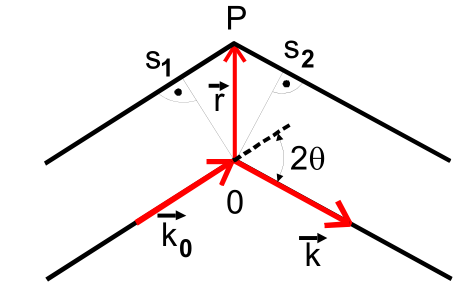
\includegraphics[width = \textwidth]{Abbildungen/streuung}
		\subcaption{Skizze, welche den Gangunterschied bei einem Streuprozess an zwei Punkten O und P zeigt.}
	\end{minipage}
	\begin{minipage}[t]{0.45\textwidth}
		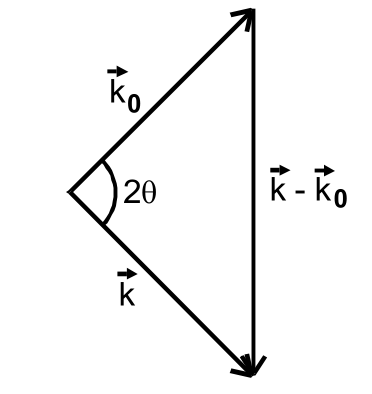
\includegraphics[width = \textwidth]{Abbildungen/streuwinkel}	
		\subcaption{Zusammenhang zwischen Streuwinkel und Wellenvektoren}
	\end{minipage}
	\caption{ Skizzierungen des Gangunterschieds $\Delta$s und der Streurichtung $\theta$ \cite{Anleitung}. }
	\label{fig:streuung}
\end{figure}
Zu beachten ist dabei, dass der Betrag der Wellenzahl der einlaufenden und der auslaufenden Welle gleich sind, wenn elsatische Streuung zu Grunde gelegt wird. Dann folgt Gleichung (\ref{eq:lambda}).
\begin{equation}
|\vec{\text{k}_0}| = |\vec{\text{k}}| = \frac{1}{\lambda}
\label{eq:lambda}
\end{equation} 
Der daraus resultierende Gangunterschied $\Delta $s aus Gleichung (\ref{eq:gangu}) lässt sich dann in die Phasendifferenz $\Delta \phi$ aus Gleichung (\ref{eq:phase}) überführen.
\begin{equation}
\Delta \text{s} = \text{s}_1+\text{s}_2 = \vec{\text{r}} \left( \frac{\vec{\text{k}}}{\text{k}} - \frac{\vec{\text{k}_0}}{k_0}  \right)
\label{eq:gangu} 
\end{equation}
\begin{equation}
\Delta \phi = 2\pi\frac{\Delta \text{s}}{\lambda} = 2\pi \vec{\text{r}} (\vec{\text{k}}-\vec{\text{k}_0})
\label{eq:phase} 
\end{equation}

Für die weitere Berechnung von f soll die Normierungsbedingung aus Gleichung (\ref{eq:normo}) gelten.
\begin{equation}
 \int_{\text{Hülle}} \rho (\vec{\text{r}}) \text{d}\text{r}^3 = \text{z}\text{e}_0
\label{eq:normo}
\end{equation}
Im Prinzip ist f eine Fouriertransformierte bezüglich der Ladungsdichteverteilung $\rho$, wie in Gleichung (\ref{eq:fourier}) zu erkennen ist,
\begin{equation}
\text{f} = \int_{\text{Hülle}} \text{e}^{-i\Delta\phi}\rho(\vec{\text{r}}) \text{d}\text{r}^3 = \int_{\text{Hülle}} \text{e}^{-i2\pi \vec{\text{r}}(\vec{\text{k}}-\vec{\text{k}_0})}\rho(\vec{\text{r}}) \text{d}\text{r}^3
\label{eq:fourier}
\end{equation}
wobei aus Abbildung (\ref{fig:streuung}) zu entnehmen ist, dass f abhängig von $\theta$ und $\lambda$ ist.
Veranschaulicht wird dies in Gleichung (\ref{eq:winkel})
\begin{equation}
|\vec{\text{k}}-\vec{\text{k}_0}| = \frac{2 \sin(\theta)}{\lambda}.
\label{eq:winkel}
\end{equation}
Damit ist die gestreute Intensität der Röntgenstrahlung an einem Atom abhängig vom Formfaktor f proportional zur Streuintensität I$_e$.\\\\
Die Streuung an einem Atom ist damit hinreichend diskutiert und muss nun auf die Streuung an einer Elementarzelle ausgeweitet werden.
Das Prinzip  einer Streuung zweier Wellen an zwei Atomen ist dabei analog zu dem vorherigen Prinzip.
Es ergibt sich wieder eine Phasendifferenz $\Delta \phi$ und eine daraus resultierende Streuamplitude aus Gleichung (\ref{eq:streuA}), die INterfenzefffekten unterlegen ist.
Dabei wird angenommen, dass ein Atom im Ursprung des Koordinatensystems liegt und die anderen im Abstand $\vec{\text{r}_j}$ folgen.
\begin{equation}
\text{A} = \sum_j \text{f}_j \text{e}^{-2\pi i \vec{\text{r}_j} (\vec{\text{k}}-\vec{\text{k}_0}) } \text{I}_e
\label{eq:streuA}
\end{equation}
Da die $\vec{\text{r}_j}$ gerade Atome auf dem Gitter sind, ist der Vektor durch die Basisvektoren darzustellen.
Wird dies ausgenutzt, so egibt sich die Strukturamplitude (\ref{eq:Struk}) der Elementarzelle.
\begin{equation}
\text{S} = \sum_j \text{f}_j \text{e}^{-2\pi i (x\vec{\text{a}}+y \vec{\text{b}}+ z \vec{\text{c}}) (\vec{\text{k}}-\vec{\text{k}_0}) } \text{I}_e
\label{eq:Struk}
\end{equation}
Nun ist noch zu beachten, dass nicht nur an zwei Atomen einer Elementarzelle, sondern an der gesamten Elementarzelle gestreut wird. 
Unter der Berücksichtigung des Huygenschen Prinzips, dass die ein und auslaufenden Wellen nur dann einen Reflex ergeben, wenn sie symmetrisch zur Netzebenennormalen liegen, ergeben sich erhebliche Einschränkungen für die sichtbaren Reflexe.
Denn Reflex ist erst dann sichtbar, wenn er durch positive Interferent verstärkt wird. Denn der Beugungsreflex eines einzelnen Atoms ist viel zu schwach.
Da aber der Röntgenstrahl an mindestens 10$^3$ Netzebenen gestreut wird, wird ein Signal durch positive Interferenz sichtbar.
Wie eine Struung an einer Netzebenenschar aussehen kann ist beispielhaft in Abbildung (\ref{fig:bragg}) gezeigt.
\begin{figure}[h]
	\centering
	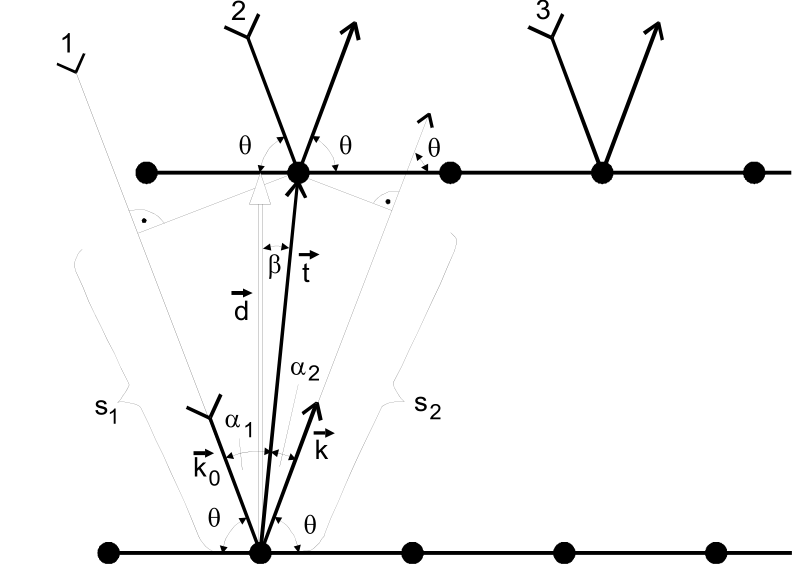
\includegraphics[width = \textwidth]{Abbildungen/bragg}
	\caption{Schematisch Struktur eines Reflexes, der der Bragg-Bedingung unterliegt}
	\label{fig:bragg}
\end{figure}
Aus der Skizze folgt für den Gangunterschied in (\ref{eq:gang2}) 
\begin{equation}
\text{n} \lambda = \Delta \text{s}_1+\Delta \text{s}_2 = \text{t}(\cos{\alpha_1}+cos{\alpha_2})
\label{eq:gang2}
\end{equation}
und daraus ergibt sich dann die Bragg-Bedingung aus Gleichung (\ref{eq:bragg}).
\begin{equation}
\text{n}\lambda = 2 \text{d} \sin{\theta}
\label{eq:bragg}
\end{equation}
Dabei ist d der Netzebenenabstand und n Element der natürlichen Zahlen $\mathbb{N}$.
Mit Hilfe von reziproken Vektoren, die senkrecht auf der Netzebene stehen und den Betrag n/$|\vec{\text{d}}|$ stellt sich die Braggbedingung wie folgt dar
\begin{equation}
 \text{n} = \vec{ \text{d}}(\vec{ \text{k}}-\vec{ \text{k}_0}).
\end{equation}
Daraus folgt dann die modifizierte Strukturamplitude in Gleichung (\ref{eq:Struk2})
\begin{equation}
\text{S}(hkl) = \sum_j \text{f}_j \text{e}^{-2\pi i (x\vec{\text{a}}+y \vec{\text{b}}+ z \vec{\text{c}}) (\vec{\text{k}}-\vec{\text{k}_0})\times (h\vec{\text{A}}+k\vec{\text{B}}+ l\vec{\text{C}}) } = \sum_j \text{f}_j \text{e}^{-2\pi i (xh+y k+ z l) }
\label{eq:Struk2}
\end{equation}
Die Großbuchstaben sind dabei die reziproken Gittervektoren zu den Basisvektoren.
\begin{equation}
s
\label{eq:g}
\end{equation}